\chapter{Calibration of sensors}
\label{ch:calibration}

\indent \indent Once the axes are properly identified, the next step is to calibrate all its sensors. The main goal of the calibration process is to transform the raw data into meaningful physical units. 

\subsection{Accelerometer calibration}
\label{subsec:acc_calibration}

\indent \indent The calibration of the accelerometers is divided in two parts according to the number of axes of the accelerometer. For the triaxial accelerometer included in the trunk unit (the box) we will use the ellipsoid fitting algorithm by Camps et al. \cite{camps_numerical_2009}. They present a theoretical and experimental method to compute gains, bias and non orthogonality factors of magnetometer and acce\-le\-ro\-me\-ter sensors. The calibration procedure involves arbitrary rotations of the MIMU, so the set of maneuvers to gather the necessary data is very simple.
\begin{itemize}
\item \textbf{Sensor Modeling}: The model of the sensor output is given by:
    \begin{equation}
    \left[
      \begin{array}{c}
        \mbox{v}_{\scriptsize \mbox{x}}(t) \\
        \mbox{v}_{\scriptsize \mbox{y}}(t) \\
        \mbox{v}_{\scriptsize \mbox{z}}(t) \\
      \end{array}
    \right]=\left[
              \begin{array}{ccc}
                \mbox{s}_{\scriptsize \mbox{x}} & 0 & 0 \\
                0 & \mbox{s}_{\scriptsize \mbox{y}} & 0 \\
                0 & 0 & \mbox{s}_{\scriptsize \mbox{z}} \\
              \end{array}
            \right]\left[
                     \begin{array}{c}
                       \mbox{m}_{\scriptsize \mbox{x}}(t) \\
                       \mbox{m}_{\scriptsize \mbox{y}}(t) \\
                       \mbox{m}_{\scriptsize \mbox{z}}(t) \\
                     \end{array}
                   \right]+\left[
                             \begin{array}{c}
                               \mbox{b}_{\scriptsize \mbox{x}} \\
                               \mbox{b}_{\scriptsize \mbox{y}} \\
                               \mbox{b}_{\scriptsize \mbox{z}} \\
                             \end{array}
                           \right]+\left[
                                     \begin{array}{c}
                                       \varepsilon_{\scriptsize \mbox{x}} \\
                                       \varepsilon_{\scriptsize \mbox{y}} \\
                                       \varepsilon_{\scriptsize \mbox{z}} \\
                                     \end{array}
                                   \right]
    \label{eq:CampsModel}
    \end{equation}
    where $\mathbf{b}=(\mbox{b}_{\scriptsize \mbox{x}}, \mbox{b}_{\scriptsize \mbox{y}}, \mbox{b}_{\scriptsize \mbox{z}})^{T}$ represents the offset, $\mbox{s}_{\scriptsize \mbox{x}}$, $\mbox{s}_{\scriptsize \mbox{y}}$, $\mbox{s}_{\scriptsize \mbox{z}}$ are the sensor gains, $\mbox{m}_{\scriptsize \mbox{x}}(t)$, $\mbox{m}_{\scriptsize \mbox{y}}(t)$, $\mbox{m}_{\scriptsize \mbox{z}}(t)$ are the components of the actual magnetic field or gravity and $\varepsilon_{x}$, $\varepsilon_{y}$, $\varepsilon_{z}$ are the components of the noise for each axis. \\
    \indent If we take into consideration the effects of non-orthogonality, then the sensor output is given by:
    \begin{equation}
    \left[
      \begin{array}{c}
        \mbox{v}_{\scriptsize \mbox{x}}(t) \\
        \mbox{v}_{\scriptsize \mbox{y}}(t) \\
        \mbox{v}_{\scriptsize \mbox{z}}(t) \\
      \end{array}
    \right]=\left[
              \begin{array}{ccc}
                \mbox{s}_{\scriptsize \mbox{xx}} & s_{\scriptsize \mbox{xy}} & s_{\scriptsize \mbox{xz}} \\
                \mbox{s}_{\scriptsize \mbox{xy}} & s_{\scriptsize \mbox{yy}} & s_{\scriptsize \mbox{yz}} \\
                \mbox{s}_{\scriptsize \mbox{xz}} & s_{\scriptsize \mbox{yz}} & s_{\scriptsize \mbox{zz}} \\
              \end{array}
            \right]\left[
                     \begin{array}{c}
                       \mbox{m}_{\scriptsize \mbox{x}}(t) \\
                       \mbox{m}_{\scriptsize \mbox{y}}(t) \\
                       \mbox{m}_{\scriptsize \mbox{z}}(t) \\
                     \end{array}
                   \right]+\left[
                             \begin{array}{c}
                               \mbox{b}_{\scriptsize \mbox{x}} \\
                               \mbox{b}_{\scriptsize \mbox{y}} \\
                               \mbox{b}_{\scriptsize \mbox{z}} \\
                             \end{array}
                           \right]+\left[
                                     \begin{array}{c}
                                       \varepsilon_{\scriptsize \mbox{x}} \\
                                       \varepsilon_{\scriptsize \mbox{y}} \\
                                       \varepsilon_{\scriptsize \mbox{z}} \\
                                     \end{array}
                                   \right]
    \label{eq:CampsModel2}
    \end{equation}
    where $\mbox{s}_{ij}$ for $i\neq j$ represent the orthogonality errors between sensor axes $i$ and $j$.

\item \textbf{Calibration Procedure}: Using the fact that the norm of the input vector $\mathbf{m}=[\mbox{m}_{\scriptsize \mbox{x}}(t)\quad \mbox{m}_{\scriptsize \mbox{y}}(t) \quad \mbox{m}_{\scriptsize \mbox{z}}(t)]^{T}$ is constant, the following relation is derived:
    \begin{equation}
    \|\mathbf{m}\|^{2}=\mbox{m}_{\scriptsize \mbox{x}}(t)^{2}+\mbox{m}_{\scriptsize \mbox{y}}(t)^{2}+\mbox{m}_{\scriptsize \mbox{z}}(t)^{2}
    \label{eq:CampsGeneral}
    \end{equation}
    \begin{equation}
    \|\mathbf{h}\|^{2}=\left(\frac{\mbox{v}_{\scriptsize \mbox{x}}(t)-\mbox{b}_{\scriptsize \mbox{x}}}{\mbox{s}_{\scriptsize \mbox{x}}}\right)^{2}+\left(\frac{\mbox{v}_{\scriptsize \mbox{y}}(t)-\mbox{b}_{\scriptsize \mbox{y}}}{\mbox{s}_{\scriptsize \mbox{y}}}\right)^{2}+\left(\frac{\mbox{v}_{\scriptsize \mbox{z}}(t)-\mbox{b}_{\scriptsize \mbox{z}}}{\mbox{s}_{\scriptsize \mbox{z}}}\right)^{2}
    \label{eq:CampsEllip}
    \end{equation}
    Equation (\ref{eq:CampsEllip}) is the parametric equation of an ellipsoid with center $\mathbf{b}$ and semi-axes $\mbox{s}_{\scriptsize \mbox{x}}, \mbox{s}_{\scriptsize \mbox{y}}$ and $\mbox{s}_{\scriptsize \mbox{z}}$. Using the system of equations formed by the various measurements at times t, we estimate the parameters through non-linear least squares minimization of the error function
    \begin{equation}
    e_{\scriptsize \mbox{p}}(t)=\|\mathbf{m}\|^{2}-\left(\mathbf{v}(t)-\mathbf{b}\right)^{T}\left(\mbox{S}^{-1}\right)^{2}\left(\mathbf{v}(t)-\mathbf{b}\right)
    \label{eq:CampsError}
    \end{equation}
    where
    \begin{equation}
    \mbox{S}^{-1}=\left[
              \begin{array}{ccc}
                1/\mbox{s}_{\scriptsize \mbox{xx}} & 1/\mbox{s}_{\scriptsize \mbox{xy}} & 1/\mbox{s}_{\scriptsize \mbox{xz}} \\
                1/\mbox{s}_{\scriptsize \mbox{xy}} & 1/\mbox{s}_{\scriptsize \mbox{yy}} & 1/\mbox{s}_{\scriptsize \mbox{yz}} \\
                1/\mbox{s}_{\scriptsize \mbox{xz}} & 1/\mbox{s}_{\scriptsize \mbox{yz}} & 1/\mbox{s}_{\scriptsize \mbox{zz}} \\
              \end{array}
            \right]
    \label{eq:CampsS}
    \end{equation}
    The cost function $e_{\scriptsize \mbox{p}}(t)$ is quadratic, and is minimized iteratively by the \emph{Le\-ven\-berg\--Mar\-quardt} algorithm (LMA) \cite{Levenberg,Marquardt}.
\end{itemize}

Long story short, if the accelerometer is placed in multiple random quasi-static positions, the gathered data should ideally describe an sphere of radius equal to the magnitude of the gravity vector. \\
\indent Therefore, the first calibration step is to gather the acceleration data which will be used to find the optimal calibration parameters. As it is said before, we need to place the unit containing the accelerometer in multiple random quasi-static positions. To do so, we put the box in a set of random positions trying to cover all the orientations. Since the transitions from one quasi-static position to other cause the accelerometer to measure linear acceleration which disrupt the gravity acceleration, we can not just take every measured point but we need to apply an algorithm which is able to detect the quasi-static instants. \\
Figure \ref{fig:acc_multiposition_signals} show the triaxial acceleration measured in each quasi-static position in addition to the undesired linear acceleration. This figure also shows the output of the quasi-static instant detection algorithm. 

\begin{figure}[H]
\centering
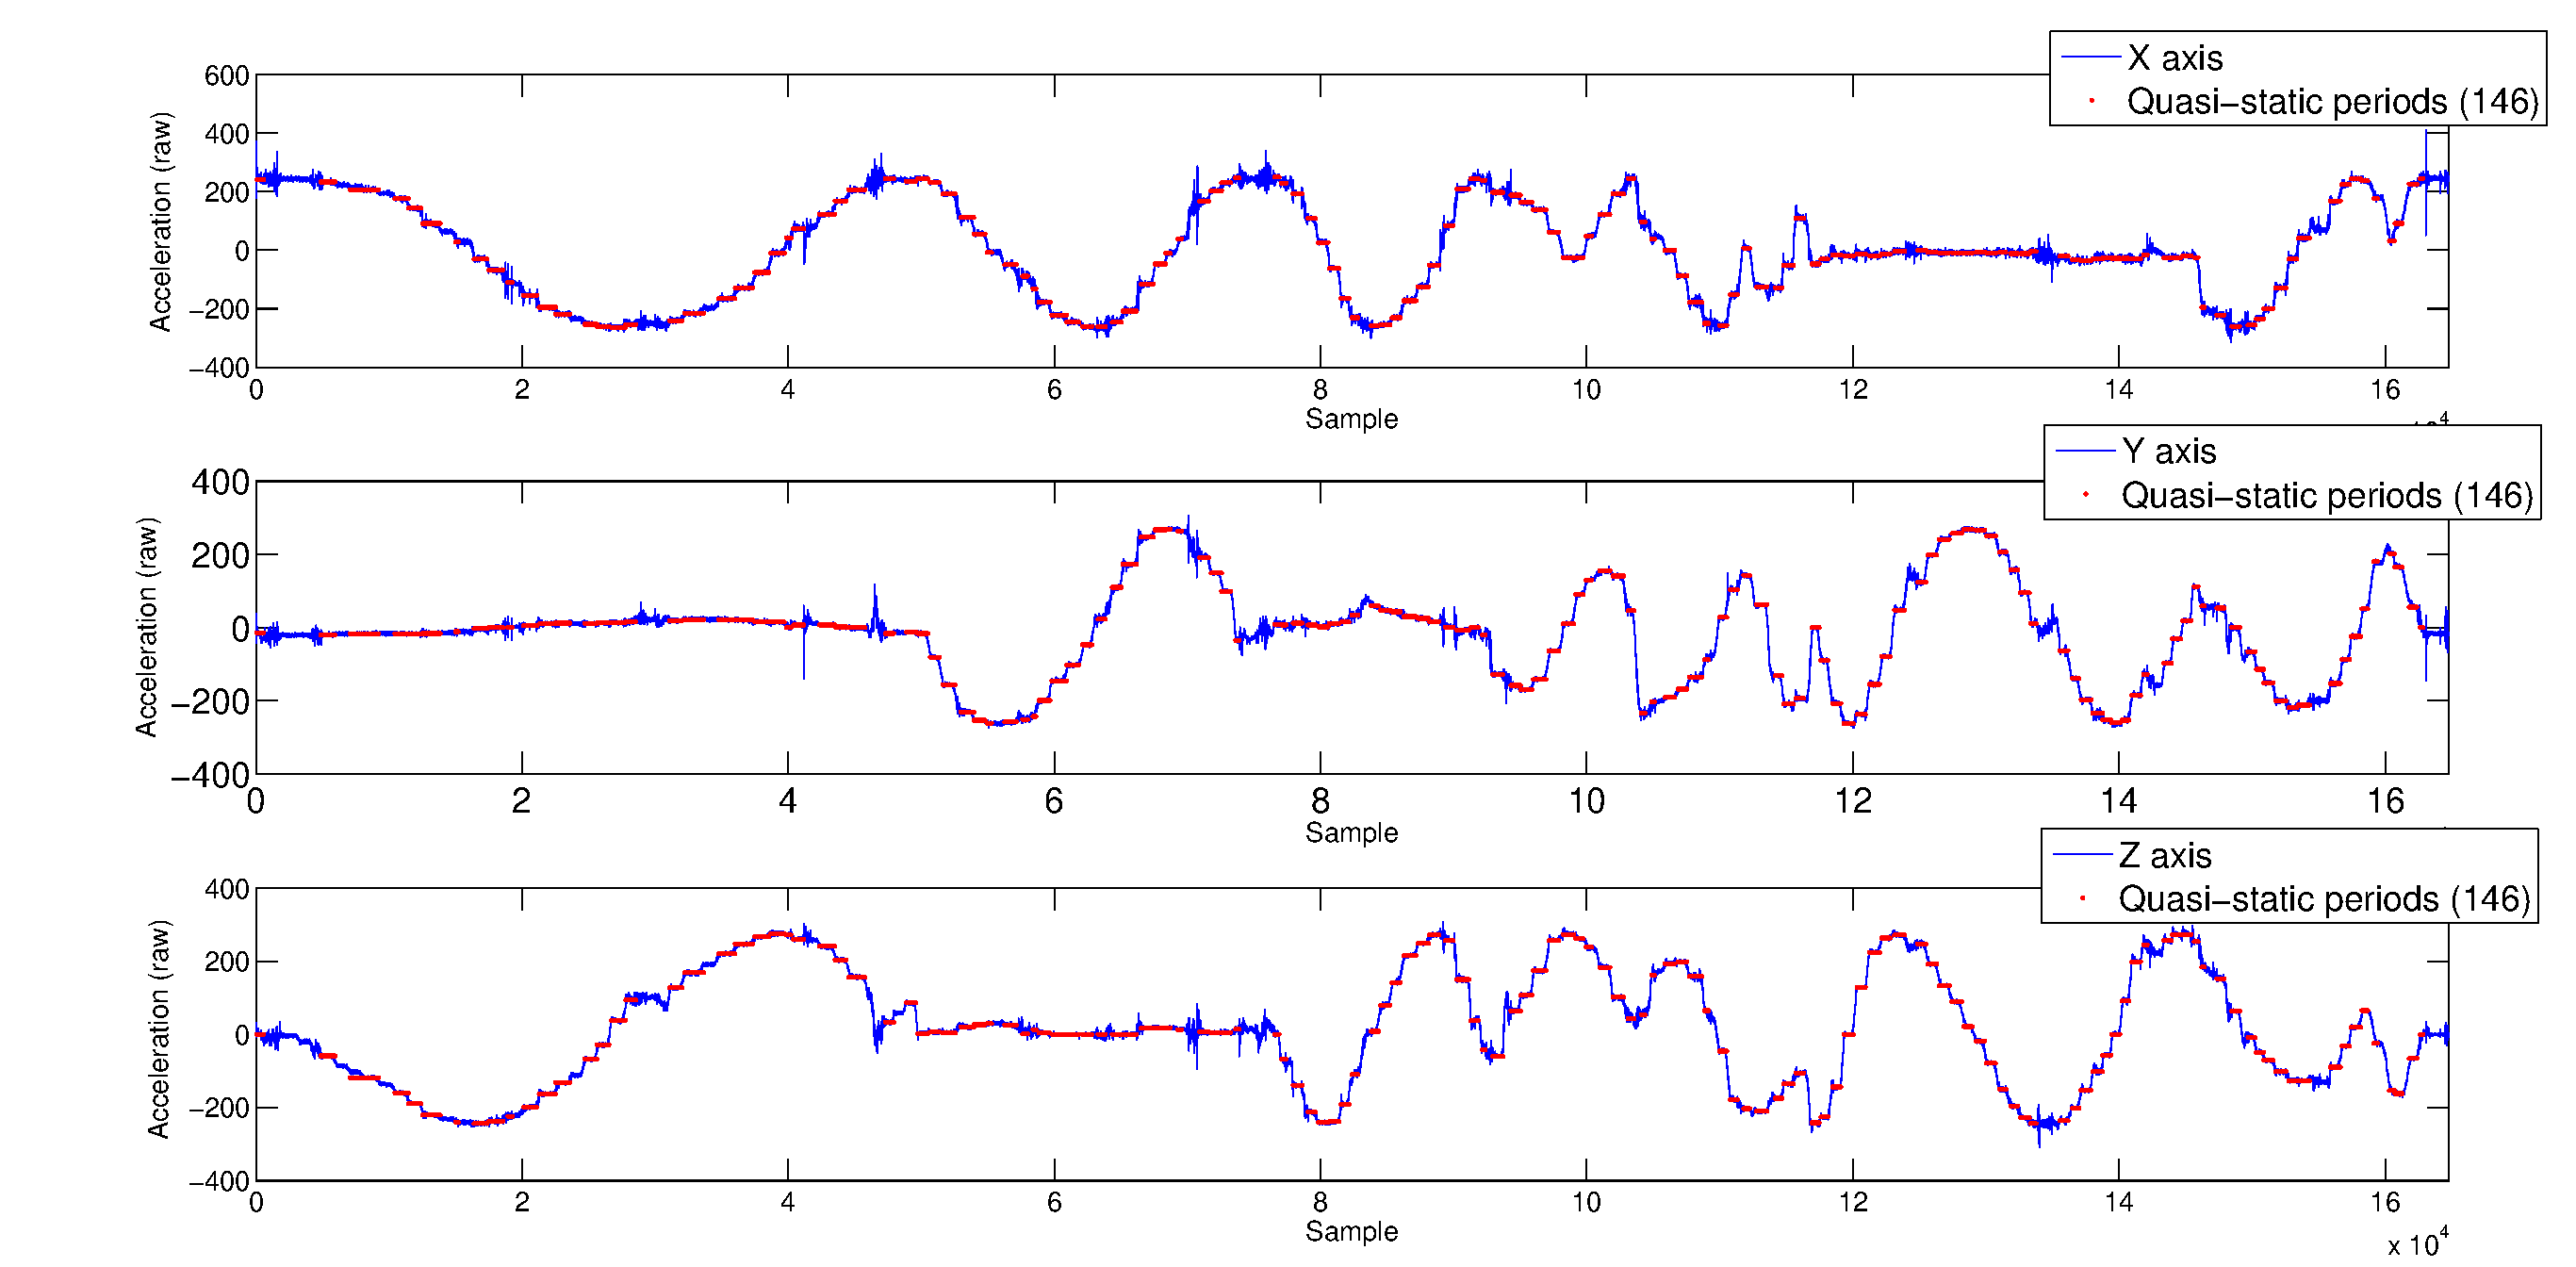
\includegraphics[width=1\textwidth]{figures/acc_multiposition_signals.eps}
\caption{Acceleration gathered during quasi-static positions and output of the detection algorithm}
\label{fig:acc_multiposition_signals}
\end{figure}

If we plot the detected quasi-static accelerations in 3D, they should cover the locus of a sphere as it is shown in figure \ref{fig:acc_multiposition_3D}

\begin{figure}[H]
\centering
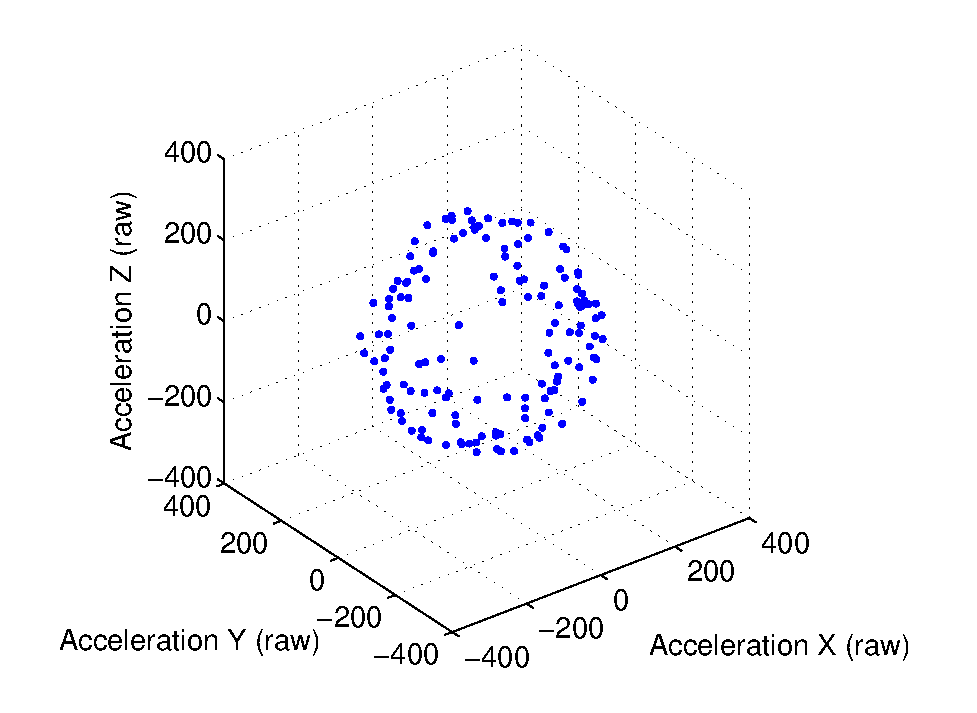
\includegraphics[width=0.6\textwidth]{figures/acc_multiposition_3D.eps}
\caption{3D representation of acceleration gathered during quasi-static positions.}
\label{fig:acc_multiposition_3D}
\end{figure}

We then feed the algorithm with these data and the calibration parameters are found. Equation \ref{eq:trunk_acc_params} shows the estimated calibration parameters for the trunk triaxial accelerometer.

\begin{gather}
\label{eq:trunk_acc_params}
S = \left[\begin{array}{ccc}
		256.68 						& -4.01\cdot10^{-5} & -2.41\cdot10^{-5} \\
		-4.01\cdot10^{-5}	&	262.74						&	-3.98\cdot10^{-7} \\
		-2.41\cdot10^{-5}	& -3.98\cdot10^{-7}	& 263.04 \\
		\end{array}\right] \\ \nonumber
\mathbf{b} = \left[-23.69\quad -6.95\quad 22.85\right]
\end{gather}

These parameters are then plugged in the following equation to obtain the calibrated triaxial acceleration:

\begin{equation}
\label{eq:cal_acceleration}
\mathbf{a}_{cal}=S^{-1}(\mathbf{a}_{raw}-\mathbf{b})
\end{equation}

where $\mathbf{a}_{cal}$ is a three dimensional vector containing the calibrated acceleration, S is the computed orthogonality matrix, $\mathbf{a}_{raw}$ is the three dimensional vector containing the raw acceleration and $\mathbf{b}$ is the computed triaxial bias vector.

Figure \ref{fig:acc_multiposition_cal_3D_4POV} shows the calibrated quasi-static accelerations. Notice how the points define now a sphere centered in the origin with a radius of 1(g).

\begin{figure}[H]
\centering
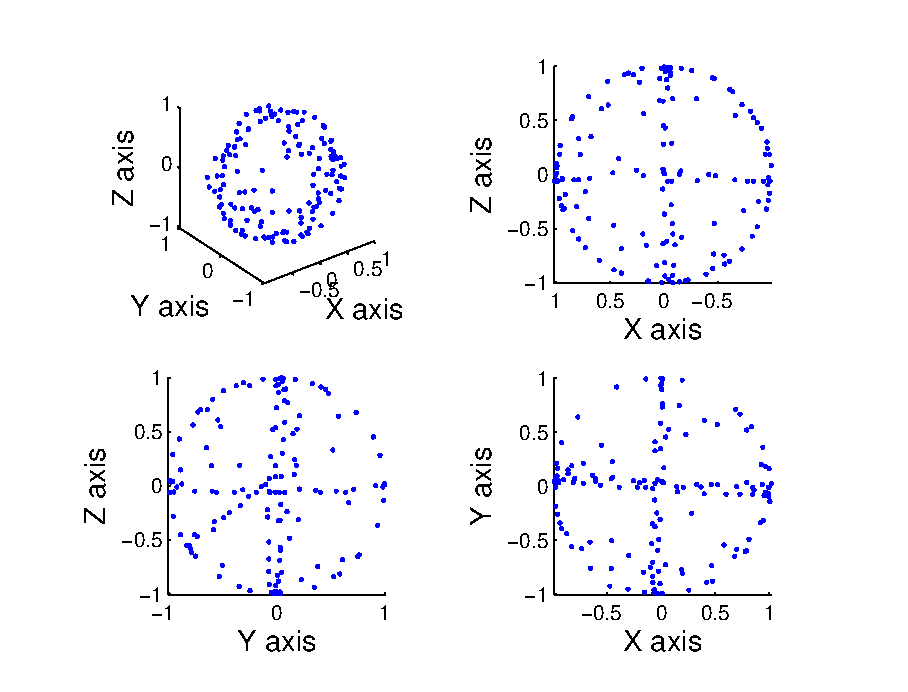
\includegraphics[width=0.8\textwidth]{figures/acc_multiposition_cal_3D_4POV.eps}
\caption{3D representation of calibrated quasi-static positions.}
\label{fig:acc_multiposition_cal_3D_4POV}
\end{figure}

For the biaxial accelerometer we could adapt the method aforementioned to two dimensions. However, the calibration maneuvers would be much more complicated since we would need to lock the unit including the accelerometer in the XZ plane and then describe a complete slow rotation to gather the quasi-static positions. \\

\indent We opted to carry out a single-axis calibration procedure which only requires to gather data from two positions for each axis. This procedure is very simple; we first set the desired axis parallel to the gravity vector and leave it in that position for a couple of seconds and we then flip it so it is anti-parallel to the gravity vector and leave it static again for another two seconds. Proceeding this way, we know the raw values corresponding to +1g and -1g respectively. Since the accelerometers included in GaitWatch's units are linear, we can then find the calibration equation in a very simple way. The calibration equation is defined as follows,

\begin{equation}
\label{eq:acc_1D_cal_equation}
a_{cal} = k\cdot a_{raw} + b
\end{equation}

where $a_{cal}$ is the calibrated acceleration, $a_{raw}$ is the raw acceleration, $k$ is the scale factor and $b$ is the bias. If we substitute the two gathered values we would have the following system of equations from which it is straight forward to find the values of $k$ and $b$,

\begin{gather}
\label{eq:acc_1D_cal_system}
1 = k\cdot a_{raw,+} + b \\ \nonumber
-1 = k\cdot a_{raw,-} + b
\end{gather}

where $a_{raw,+}$ and $a_{raw,-}$ are the gathered raw accelerations in the parallel and anti-parallel positions respectively. \\

\indent The units placed on the shanks and the thighs contain a biaxial accelerometer (X,Z) so we can put the unit in the four required positions (two for each axis) and then apply the quasi-static positions detector to extract the values in these positions. \\

\indent Figure \ref{fig:acc_raw_4_positions} shows the gathered raw acceleration in such four positions and the extracted quasi-static values for the accelerometer in the left shank unit. 

\begin{figure}[t]
\centering
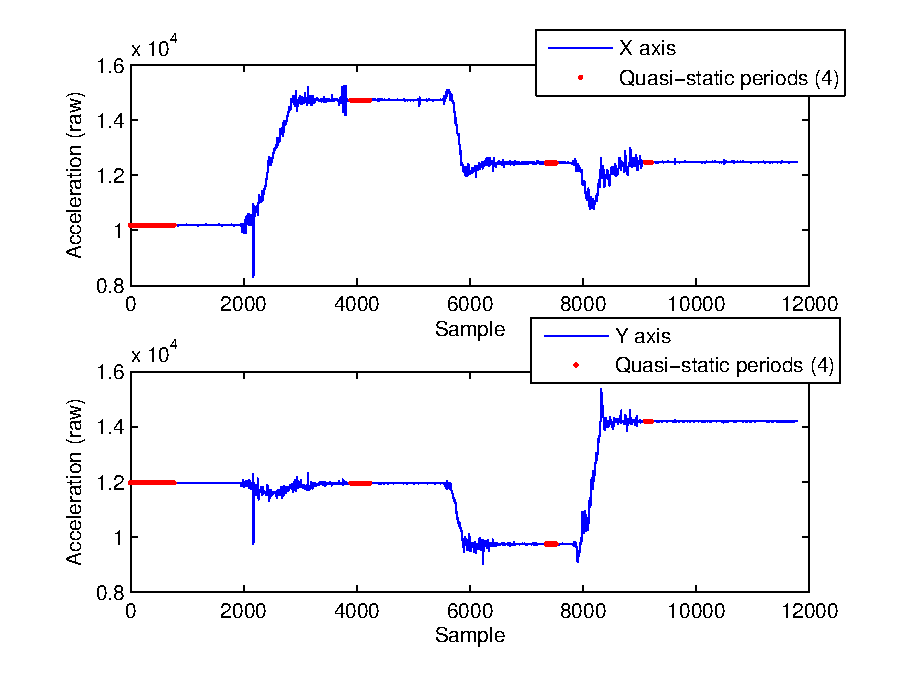
\includegraphics[width=0.8\textwidth]{figures/acc_raw_4_positions.eps}
\caption{Raw acceleration gathered when both axes X and Z are placed parallel and anti-parallel to the gravity vector.}
\label{fig:acc_raw_4_positions}
\end{figure}

Using this procedure the calibration parameters are found for all the units. Table \ref{tab:acc2D_cal_params} shows them. 

\begin{table}[H]\footnotesize
\caption{Calibration parameters of biaxial accelerometers (valid as of December the 10th, 2013).}
	\centering
		\begin{tabular}{|c|c|c|c|}\hline
		\label{tab:acc2D_cal_params}
		Unit				& Axis 	& Scale factor 	& Bias 	\\ \hline
		Left shank 	& X			& 4.45e-04			& -5.59 \\
		Left shank 	& Z			& 4.49e-04			& -5.36 \\
		Left thigh	& X			& 4.58e-04			& -5.76 \\
		Left thigh	& Z			& 4.74e-04			& -5.70 \\
		Right shank & X			& 4.38e-04			& -5.50 \\
		Right shank & Z			& 4.77e-04			& -5.72 \\
		Right thigh & X			& 4.36e-04			& -5.44 \\
		Right thigh & Z			& 4.43e-04			& -5.34 \\ \hline
		\end{tabular}
\end{table}

\subsection{Magnetometer calibration}
\label{subsec:mag_calibration}

\indent \indent The calibration of the triaxial magnetometer is also based on the algorithm by Camps et al. used for the accelerometer calibration. In this case, we only need to change the data gathering maneuvers and the value of the magnitude of the reference vector (which in this case is the Earth's magnetic field vector).\\

\indent The maneuvers are much simpler in this case since the magnetometer is not affected by the linear acceleration. Therefore, we can freely move the magnetometer at any speed trying to cover the most possible space. Figure \ref{fig:mag_raw_3D} shows the 3D representation of the raw magnetic field measured carrying these maneuvers. 

\begin{figure}[t]
\centering
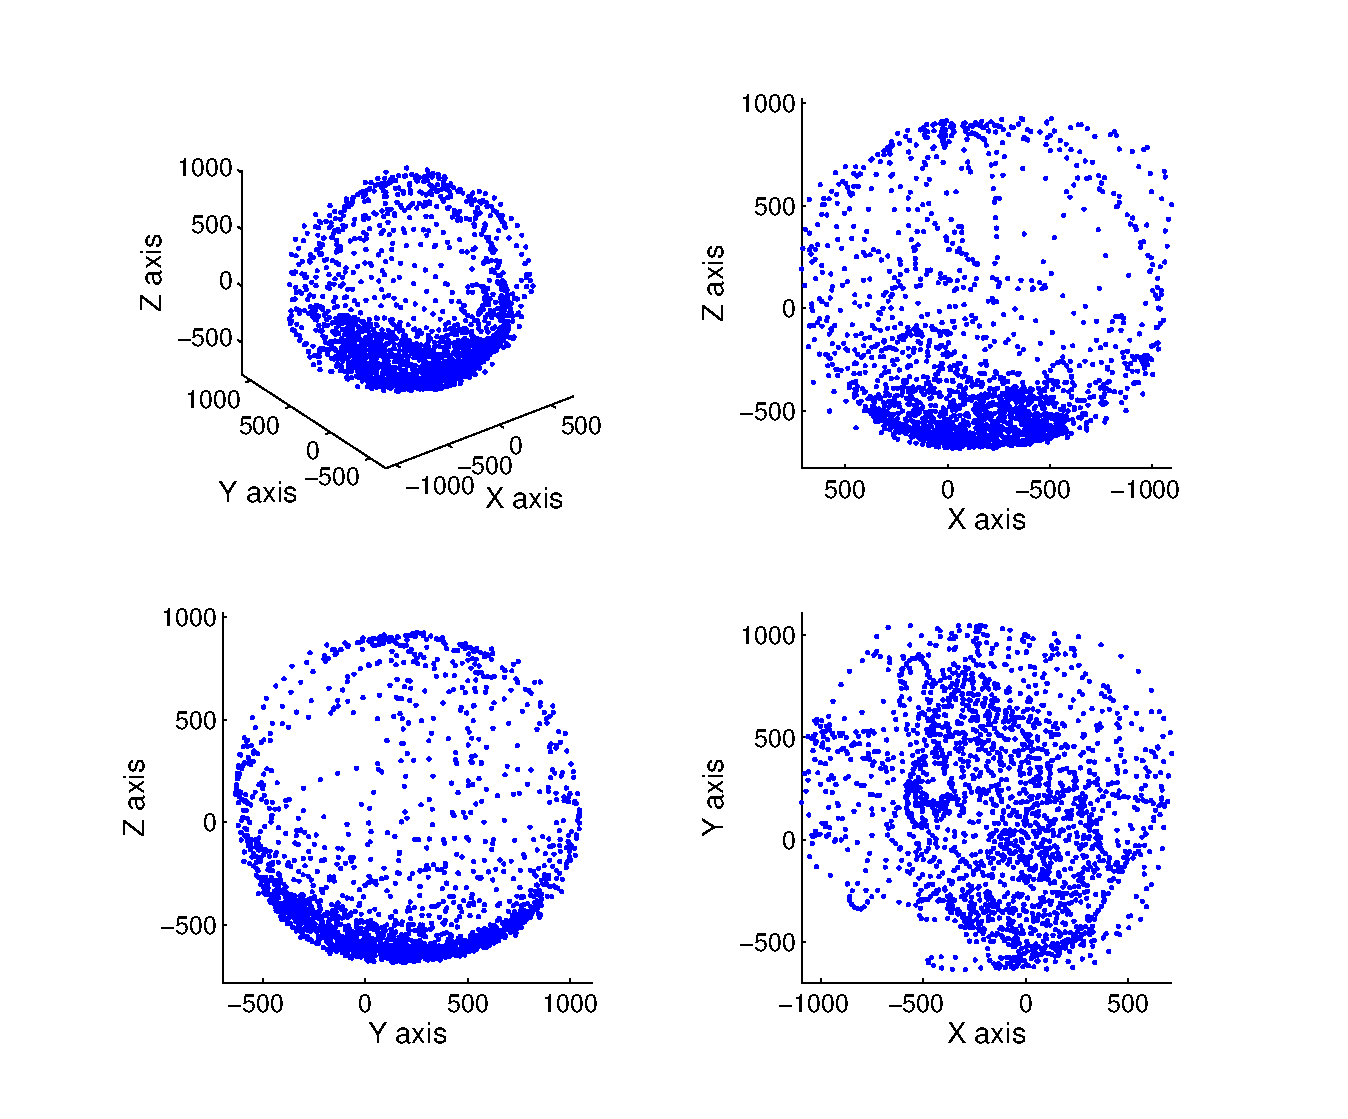
\includegraphics[width=0.8\textwidth]{figures/trunk_rawMag3D_4POV.eps}
\caption{Raw magnetic field gathered by randomly moving the trunk unit containing the magnetometer.}
\label{fig:mag_raw_3D}
\end{figure}

Ideally, these data should describe an sphere centered in the origin with a radius given by the magnitude of the local Earth's magnetic field. By checking the Magnetic field calculator from the American National Geophysical Data Center \cite{center_ngdc}, we can obtain the value for Munich, which is 0.482352 Gauss. We then feed the algorithm with the data shown in figure \ref{fig:mag_raw_3D} and the calibration parameters are computed. Analogously to the accelerometer, the calibrated magnetic field is found applying the following equation,

\begin{equation}
\label{eq:cal_mag}
\mathbf{h}_{cal}=S^{-1}(\mathbf{h}_{raw}-\mathbf{b})
\end{equation}

where again $\mathbf{h}_{cal}$ is a three dimensional vector containing the calibrated magnetic field, S is the computed orthogonality matrix, $\mathbf{h}_{raw}$ is the three dimensional vector containing the raw magnetic field and $\mathbf{b}$ is the computed triaxial bias vector. If we apply this equation to the raw values used to compute the parameters, we can see how they now define a sphere centered in 0 and with radius 0.482352 Gauss (figure \ref{fig:mag_cal_3D}).

\begin{figure}[H]
\centering
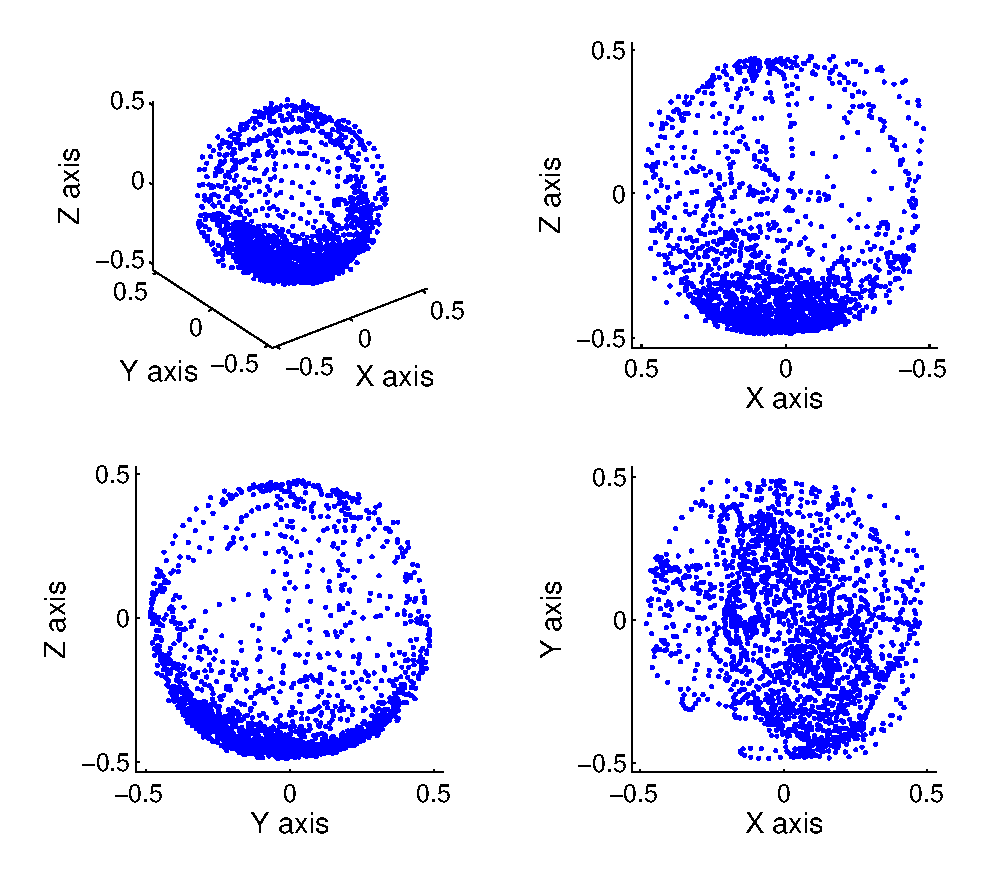
\includegraphics[width=0.5\textwidth]{figures/trunk_calMag3D_4POV.eps}
\caption{Calibrated magnetic field gathered by randomly moving the trunk unit containing the magnetometer.}
\label{fig:mag_cal_3D}
\end{figure}

Figure \ref{fig:trunk_rawVsCal} shows the raw and calibrated signals for all the three axes of the magnetometer included in the trunk's unit.

\begin{figure}[H]
\centering
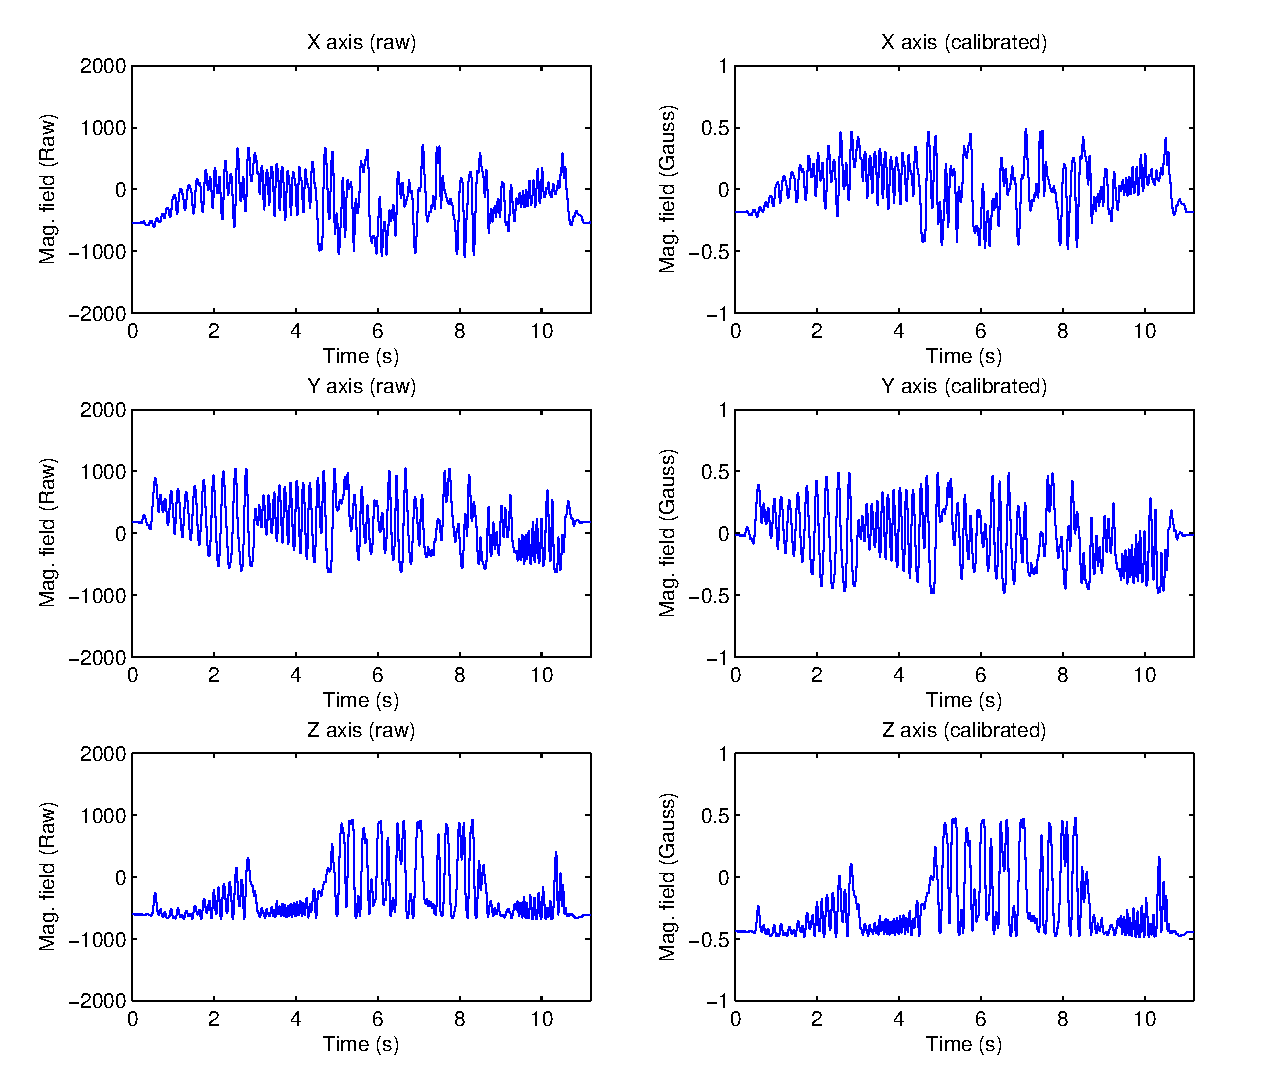
\includegraphics[width=0.7\textwidth]{figures/trunk_rawVsCal.eps}
\caption{Calibrated magnetic field vs. raw magnetic field gathered by randomly moving the trunk unit containing the magnetometer.}
\label{fig:trunk_rawVsCal}
\end{figure}

The calibration parameters (valid as of December the 10th, 2013) of the magnetometer in the trunk unit are listed below 

\begin{gather}
\label{eq:mag_cal_params}
S = \left[\begin{array}{ccc}
		1.75\cdot10^{3} 	& -3.46\cdot10^{-8} & -3.04\cdot10^{-6} \\
		-3.46\cdot10^{-8}	&	1.97\cdot10^{3}	 & 1.42\cdot10^{-5} \\
		-3.04\cdot10^{-5}	& 1.42\cdot10^{-6} & 1.83\cdot10^{3}  \\
		\end{array}\right] \\ \nonumber
\mathbf{b} = \left[14.86\quad 102.43\quad -45.04\right]
\end{gather}

\subsection{Gyroscope calibration}
\label{subsec:gyro_calibration}

\indent \indent The gyroscope is the last remaining kind of sensor to be calibrated. The most accurate way to calibrate a gyroscope is to subject it to different known rotation speeds and then associating them to the raw gathered values to obtain a calibration equation. If a variable rate table is not available, we can use simpler equipment and subject the gyroscope to known rotations instead of known angular rates. To calibrate each one of the axis we need to build a device like the one shown in figure \ref{fig:gyro_turn_device}. This device should allow the rotation of the unit containing the gyroscope around $180^{\circ}$ (other configurations of the device allowing different known rotations are also valid). 

\begin{figure}[H]
\centering
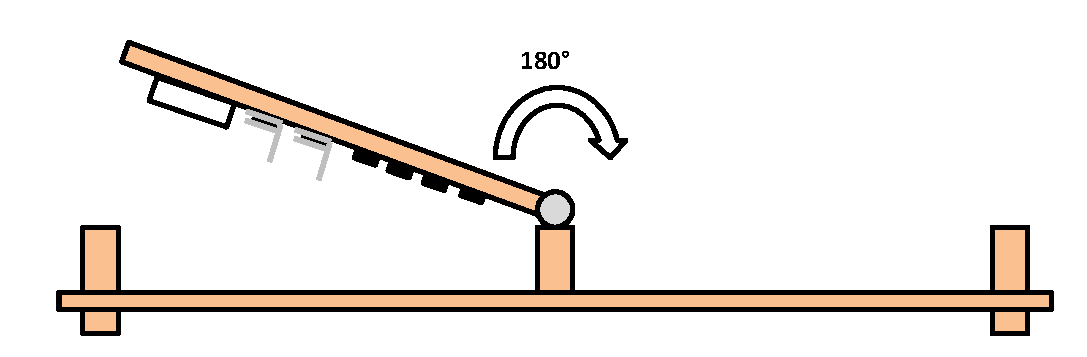
\includegraphics[width=0.8\textwidth]{figures/gyro_turn_device}
\caption{Gyroscope calibration device.}
\label{fig:gyro_turn_device}
\end{figure}

Once the calibration device is ready, the calibration maneuvers are not complicated. Each of the units should be attached to the surface of the device and then we need to carry out a set of $180^{\circ}$ rotations (at least 5). \\

\indent To compute the calibration parameters we are going to use the fact that the integration of the angular speed leads to an angle displacement. Therefore, if we subject the gyroscope to a known rotation ($180^{\circ}$ degrees in this case), we can apply the following equations to find the scale factor,

\begin{gather}
u_{raw} = k\cdot \omega + b \label{eq:gyro_cal1}\\
\omega = \frac{u_{raw}-b}{k} \label{eq:gyro_cal2}\\
u_{raw,corr} = u_{raw}-b \label{eq:gyro_cal3}\\
\int{\omega dt} = \frac{\int{u_{raw,corr} dt}}{k} \label{eq:gyro_cal4}\\
\Omega = \int{\omega dt} \label{eq:gyro_cal5}\\
\theta = \int{u_{raw,corr} dt} \label{eq:gyro_cal6}\\
\Omega = \frac{\theta}{k} \label{eq:gyro_cal7}\\
k = \frac{\theta}{\Omega} \label{eq:gyro_cal8}\\
\end{gather}

\noindent where $u_{raw}$ is the raw gathered angular rate, $\omega$ is the actual angular rate (in physical units), $k$ is the scale factor and $b$ is the bias. In this case $\Omega = 180^{\circ}$ and $\theta$ is the integrated raw gathered angular rate (corrected in bias) during the rotation of $180^{\circ}$. We can see that prior to the integration of the raw angular rate we need to subtract the bias. \\

The bias is easily found by leaving the units in a static position before starting the rotation and then visually inspecting the gathered signal. To take into account the effects of noise, we compute the mode of all the samples gathered while the sensors are static. \\

From a practical point of view, the Matlab calibration routine first displays the gathered raw angular rate signal and asks the user to select the initial and final points of the static period as it is shown in figure \ref{fig:gyro_cal_routine_bias}.

Once the bias is found, we need to tell the routine each one of the starting and ending points of the rotations so it knows the initial and final time instants of the integration. To do so we use the \textit{datacursor}. It is important to only select the positive rotations (as indicated in figure \ref{fig:gyro_cal_routine_sf}), that is, those in which the angular rate first increases and then decreases. The routine will then integrate the selected segments of the signal and average the computed scale factor for each one of them. 

The calibrated angular rate is finally found by substituting the computed calibration parameters in equation (\ref{eq:gyro_cal2}).

\begin{figure}[H]
\centering
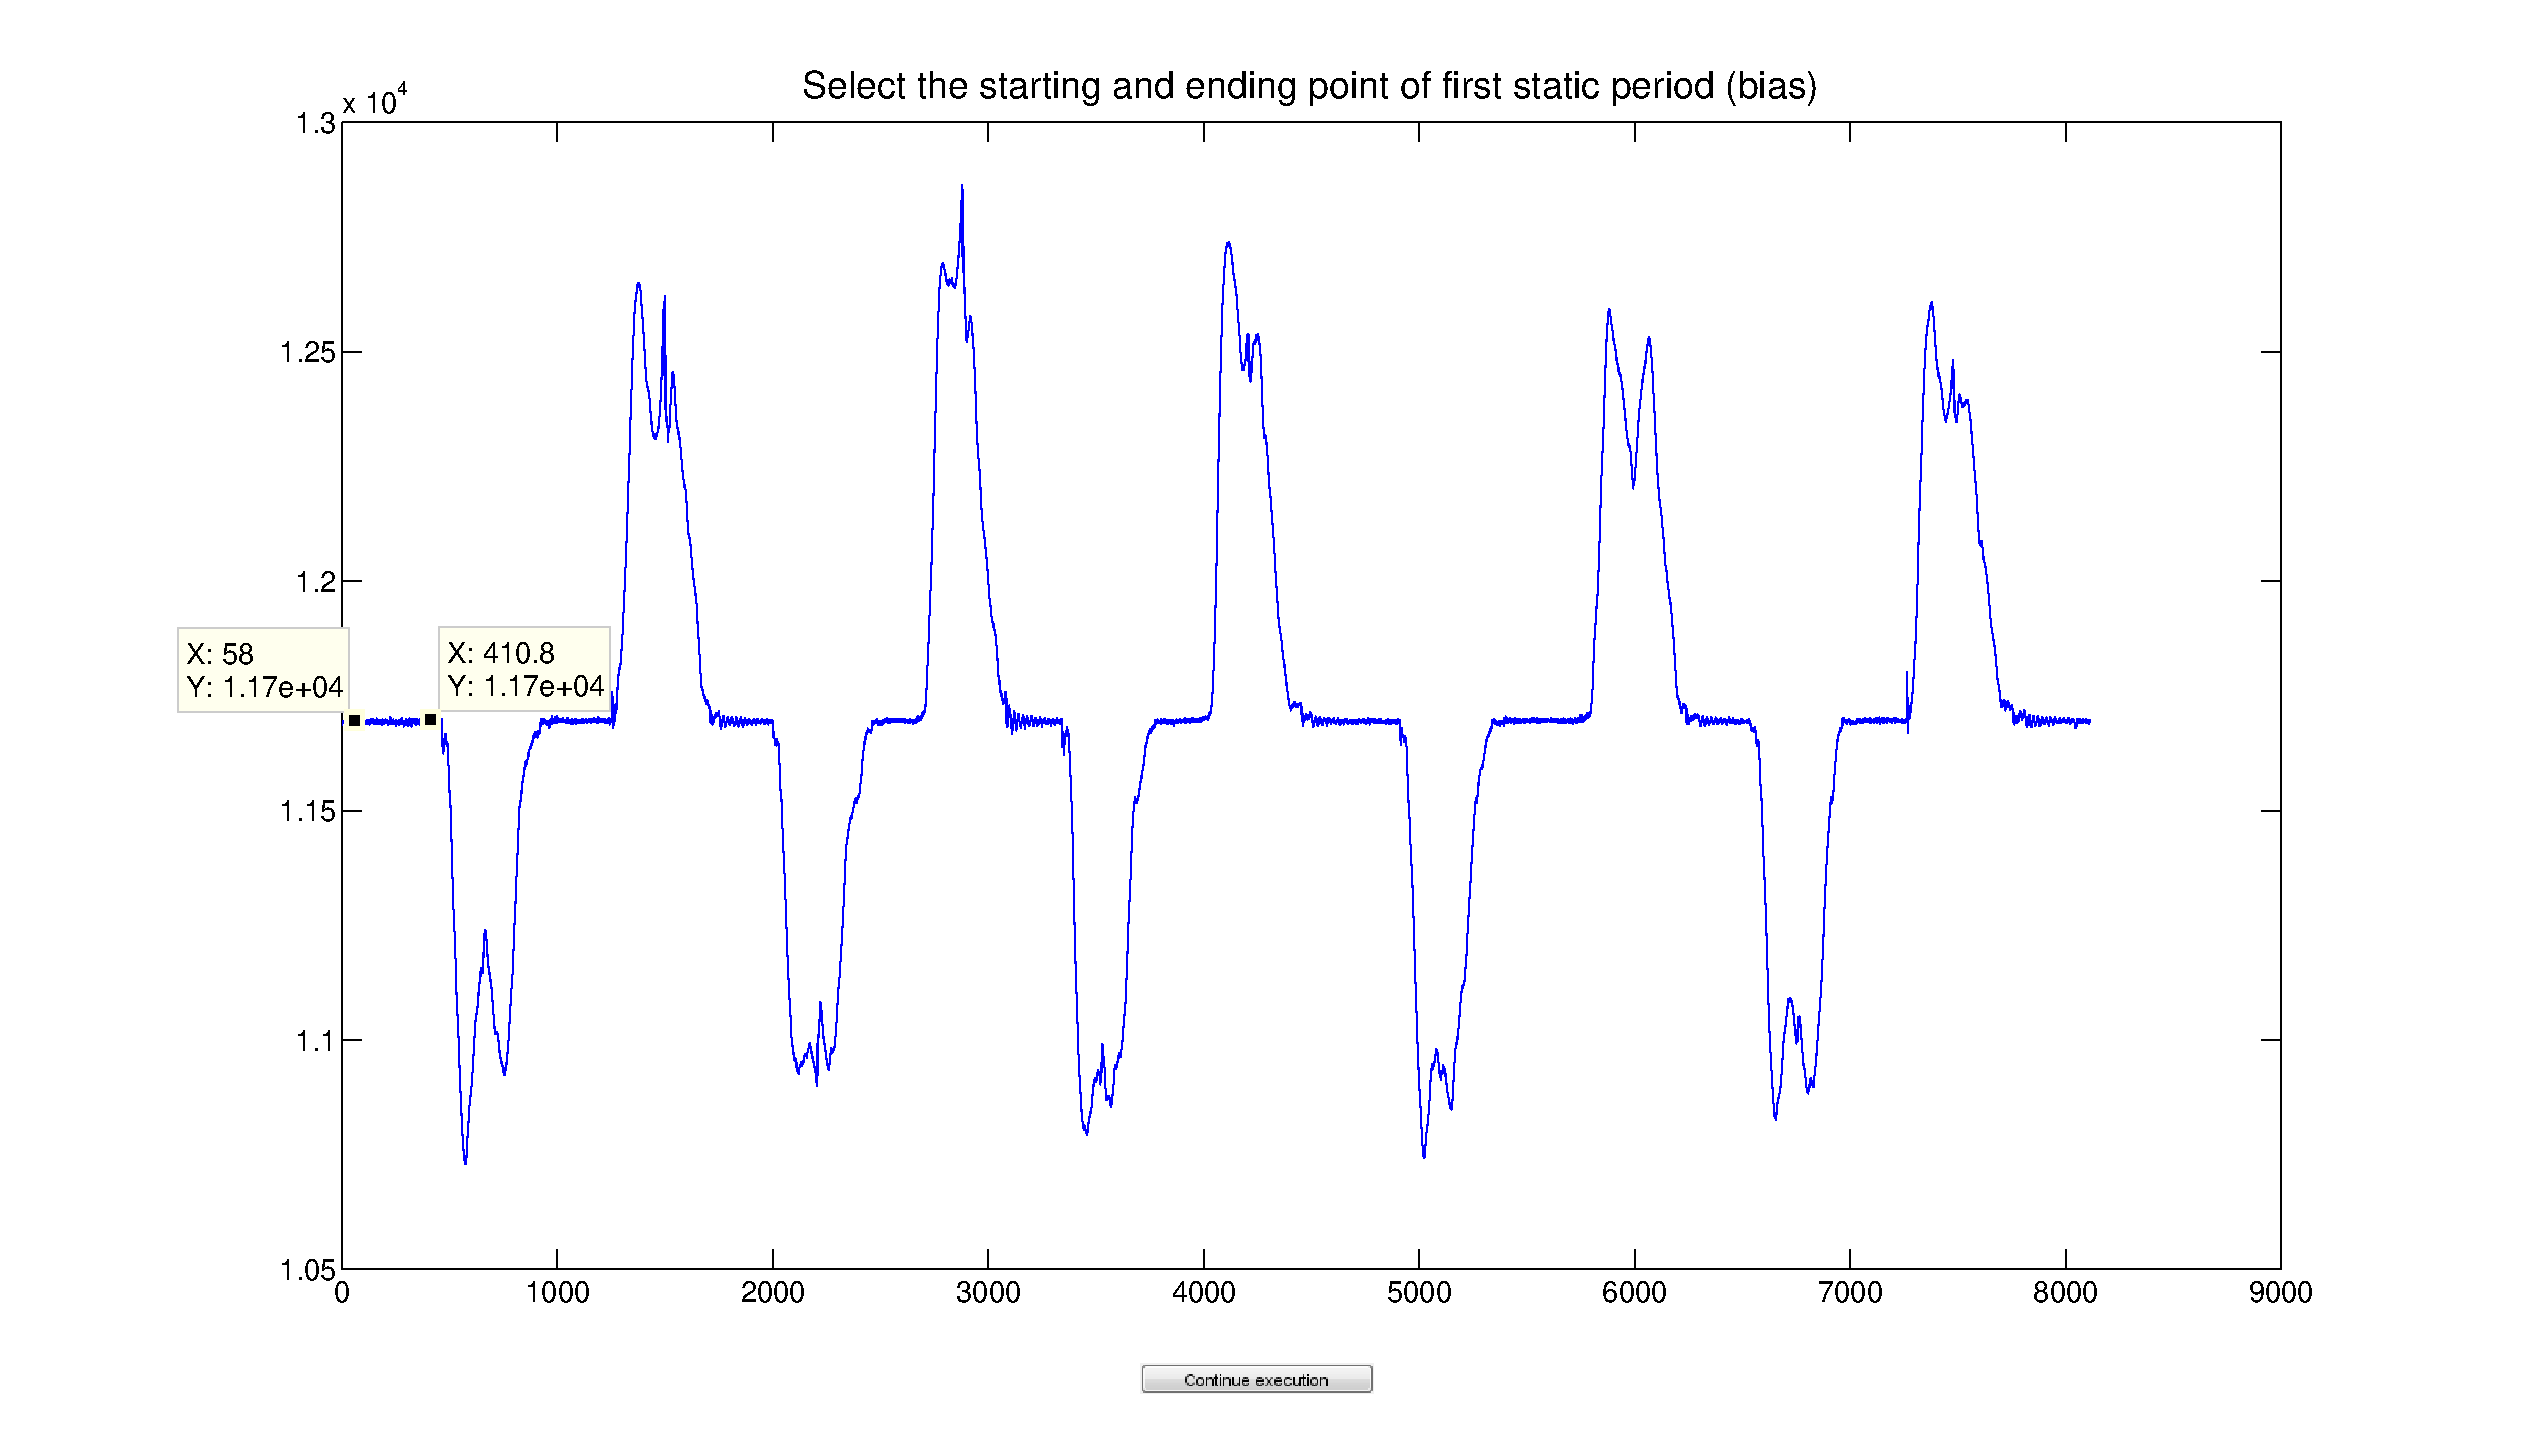
\includegraphics[width=1\textwidth]{figures/gyro_cal_routine_bias.eps}
\caption{Gyroscope calibration routine: selection of static period to compute bias.}
\label{fig:gyro_cal_routine_bias}
\end{figure}

\begin{figure}[H]
\centering
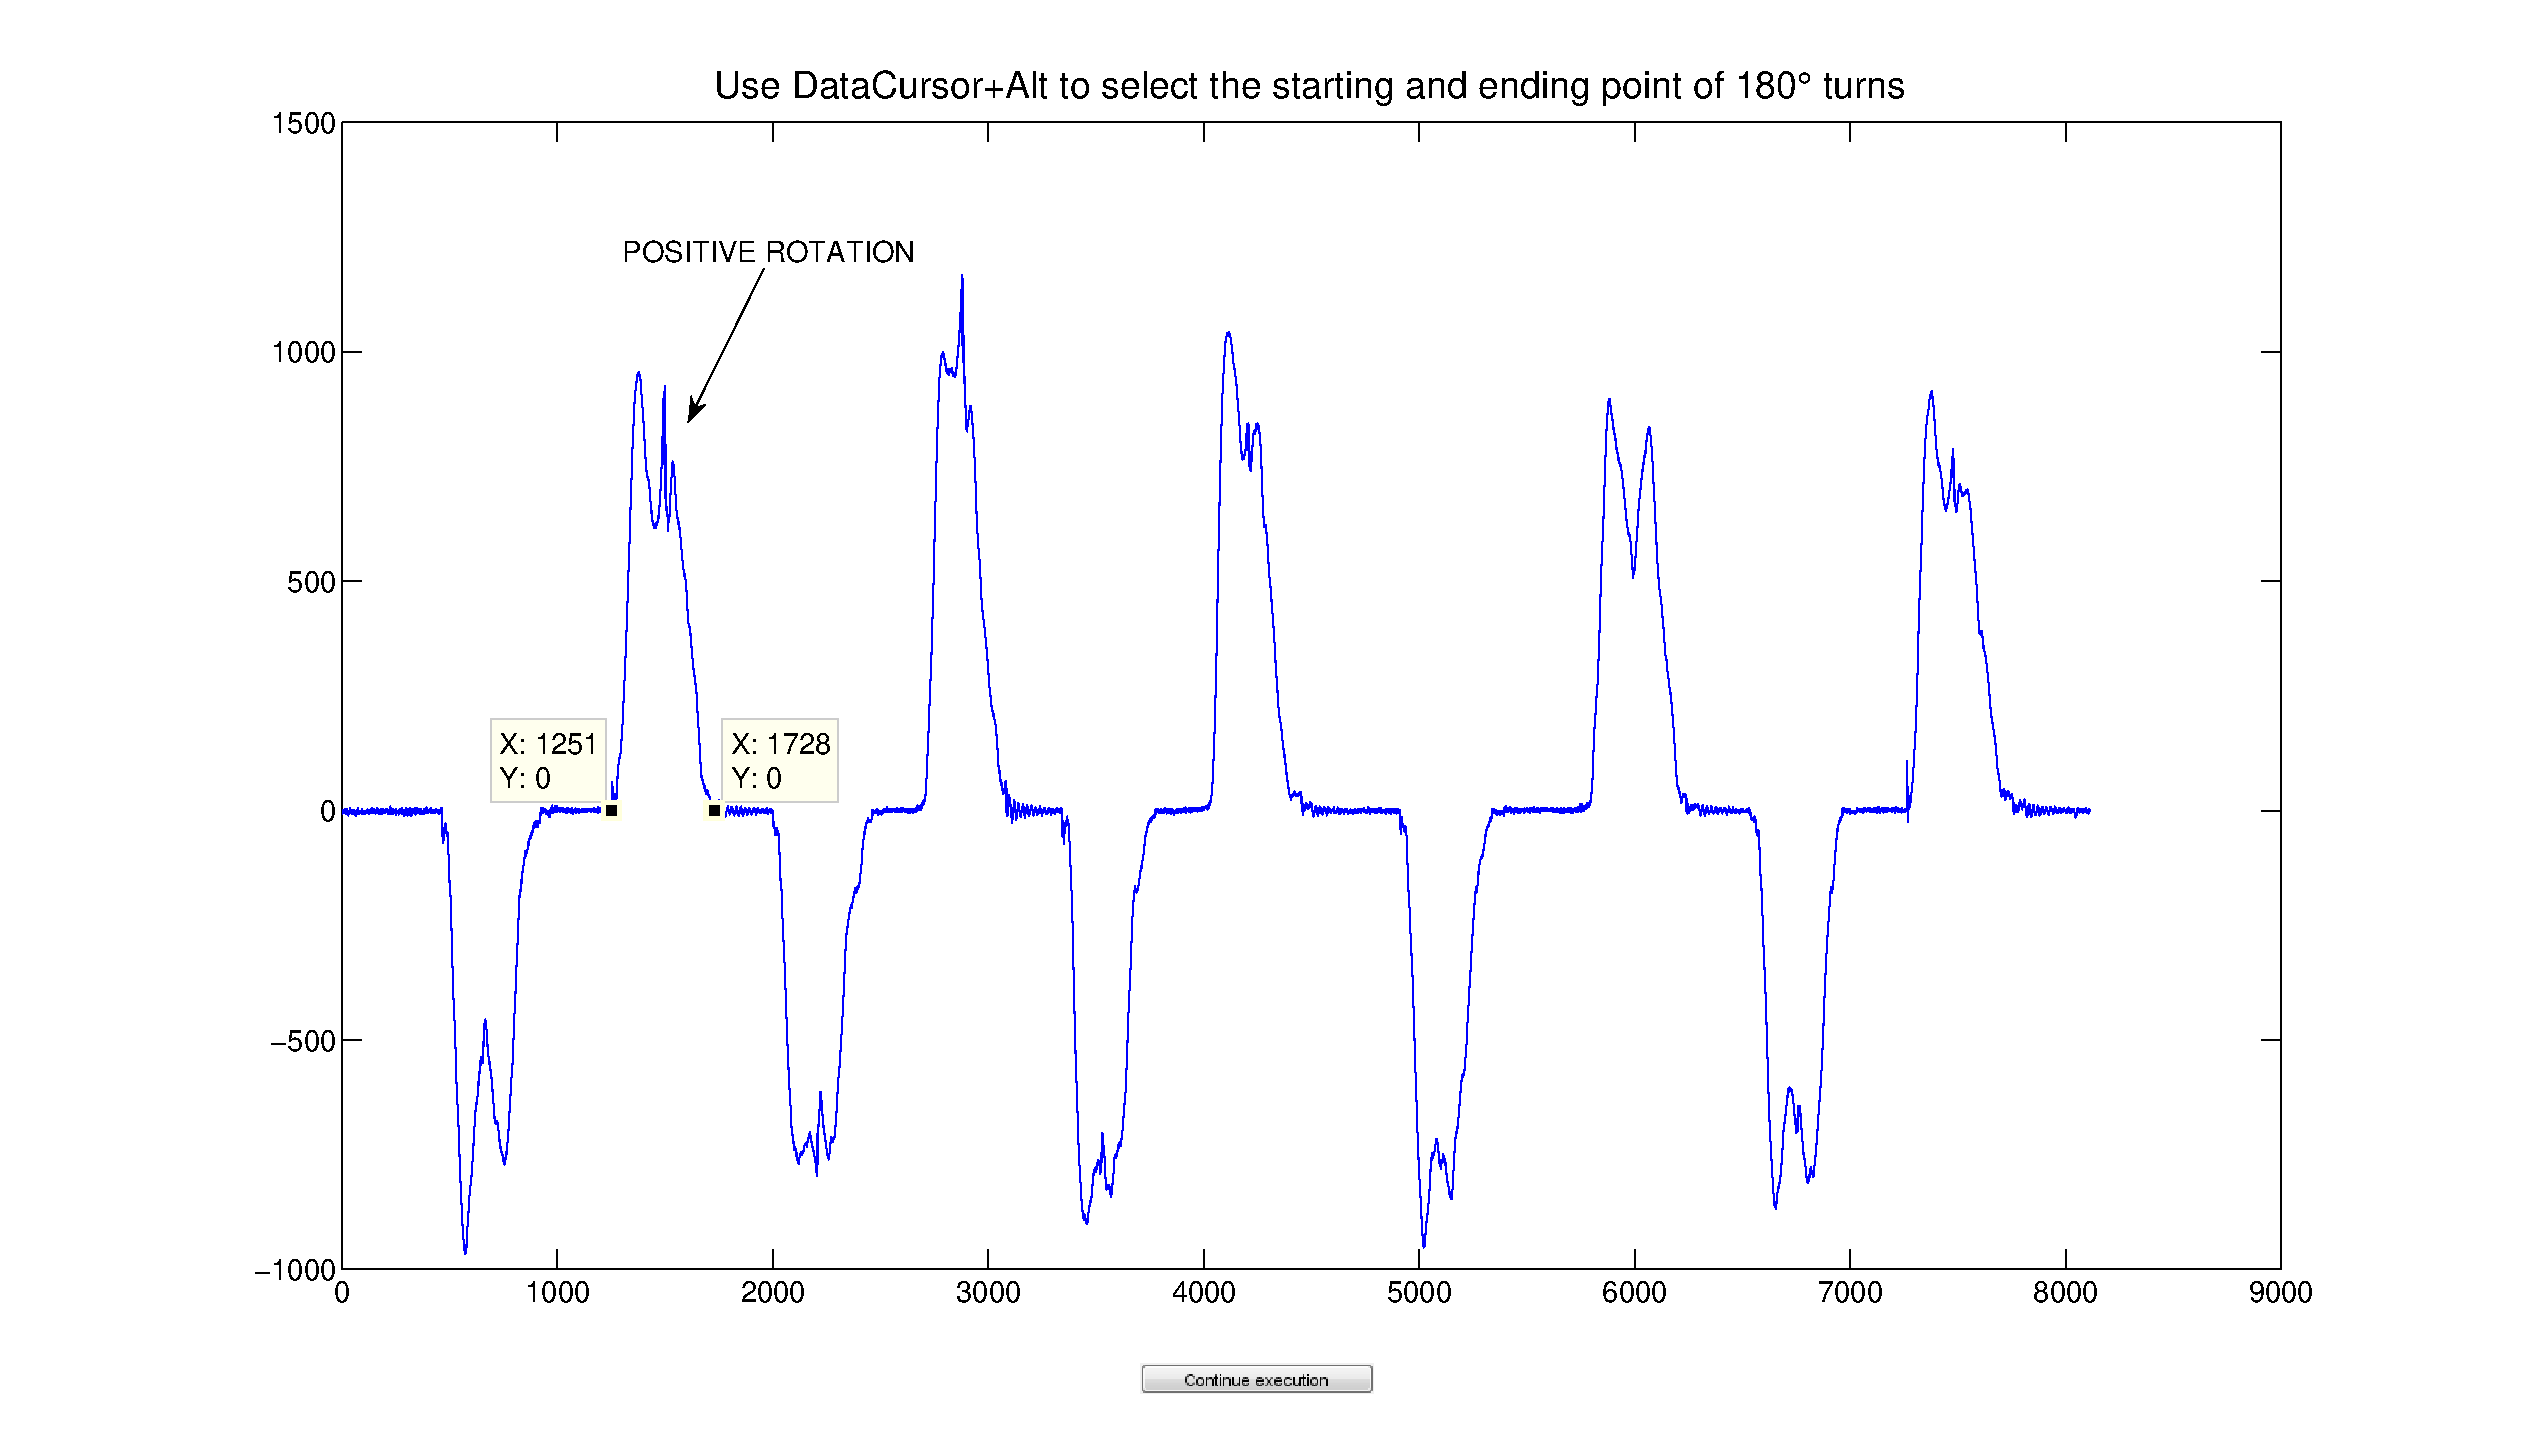
\includegraphics[width=1\textwidth]{figures/gyro_cal_routine_sf.eps}
\caption{Gyroscope calibration routine: selection of positive rotations to compute scale factor.}
\label{fig:gyro_cal_routine_sf}
\end{figure}

Table \ref{tab:gyro_cal_params} lists the computed calibration parameters for all GaitWatch's gyroscopes.

\begin{table}[H]\footnotesize
\caption{Calibration parameters of gyroscopes (valid as of December the 10th, 2013).}
	\centering
		\begin{tabular}{|c|c|c|c|}\hline
		\label{tab:gyro_cal_params}
		Unit				& Axis 	& Scale factor 	& Bias 	\\ \hline
		Left shank 	& Y			& -5.84					& 11591 \\
		Left thigh	& Y			& -6.36					& 11720 \\
		Right shank & Y			& -5.95					& 11618 \\
		Right thigh & Y			& -6.40					& 11740 \\ 
		Left arm	  & X			& -5.89					& 12087 \\
		Left arm		& Y			& 5.75					& 10937 \\
		Right arm   & X			& -6.02					& 11543 \\
		Right arm   & Y			& 5.64					& 11415 \\ 
		Trunk				& X			& -16.15				& -10		\\
		Trunk				& Y			& 16.02					& 62		\\	
		Trunk				& Z			& 16.23					& 31		\\
		\hline
		\end{tabular}
\end{table}

\subsection{Wrap-up}
\label{subsec:cal_wrapup}
\indent \indent As a final summary, once all the calibration parameters from all the sensors are computed, we only need to apply the following equations,

\begin{itemize}
\item \textbf{Accelerometer}:
	\begin{itemize}
	\item \textit{Triaxial accelerometer}:
		\begin{equation}
		\label{eq:cal_acceleration_summary}
		\mathbf{a}_{cal}=S^{-1}(\mathbf{a}_{raw}-\mathbf{b})
		\end{equation}
	\item \textit{Biaxial accelerometer}:
		\begin{equation}
		\label{eq:acc_1D_cal_equation_summary}
		a_{cal} = k\cdot a_{raw} + b
		\end{equation}
	\end{itemize}
\item \textbf{Magnetometer}:
	\begin{equation}
	\label{eq:cal_mag_summary}
	\mathbf{h}_{cal}=S^{-1}(\mathbf{h}_{raw}-\mathbf{b})
	\end{equation}
\item \textbf{Gyroscope}:
\begin{equation}
\label{eq:gyro_cal2_summary}
\omega_{cal} = \frac{u_{raw}-b}{k} 
\end{equation}
\end{itemize}